\documentclass[a4paper,10pt]{article}
%\documentclass[a4paper,10pt]{scrartcl}

\usepackage[authoryear]{natbib}
\usepackage[utf8]{inputenc}
\usepackage{hyperref}
\usepackage{multirow}
\usepackage{pdfpages}

\title{ICCAT Software Catalogue}
\author{}
\date{}

\pdfinfo{%
  /Title    ()
  /Author   ()
  /Creator  ()
  /Producer ()
  /Subject  ()
  /Keywords ()
}

\begin{document}
\maketitle

\section*{Introduction}

Action 1.3 of the Strategic Plan is to reinvigorate the Working Group of the Stock Assessment Catalogue (WGSAC) and review the protocols of inclusion and updating the software used for stock assessments while maintaining a historic repository of version control. The current catalogue application form can be found in appendix 1. 

The first step in this process was to review current procedures by circulating a questionnaire to rapporteurs of stock assessment working groups to summarise software currently used by the SCRS and to canvass their views on reinvigoration. A second questionnaire was sent to software developers in order to ensure that innovation is encouraged and that catalogue requirement do not become burdensome.

This document summarises the survey results and based on these proposes a new protocol for including software in the catalogue. This is proposed as a \textit{straw person} and to evaluate the new procedure rapporteurs are asked to use it to evaluate the latest version of ASPIC Version 7.01 \footnote{\url{http://www.mhprager.com/aspic.html}}.

The purpose of the catalouge is not to evaluate the relative merits of a method, but to provide a check list of whether the software works as intended and is adequately documented.  Inclusion of a particular computer program in the ICCAT software catalogue does not guarantee that the software is free of bugs, nor does it imply any sort of institutional endorsement for its use. Inclusion in the catalogue is simply a way of documenting what steps, if any, the programmer has taken to ensure that the program does what it purports to do. Following the establishment of the catalogue various global initiative related to stock assessment have been implemented. For example the Strategic Initiative on Stock Assessment Methods (SISAM\footnote{\url{http://www.ices.dk/community/groups/Pages/SISAM.aspx}}) aims to help advance knowledge on the use and development of stock assessments and guide scientists to the most appropriate stock assessment software/methods. The Working Group on Stock Assessment Methods (WGSAM) recommended working with SISAM to ensure that the ICCAT software catalogue becomes part of a worldwide repository of stock assessment methods. 

\section*{Strategic Plan}

At its 2014 meeting, the SCRS adopted a Science Strategic Plan for the functioning and orientation of the SCRS. This included \textbf{Action 1.3 Consolidate the stock assessment catalogue to ensure the best use of models that should be fully documented}. To execute this action three strategies were specified, namely to

\begin{itemize}
 \item  Update the current Stock Assessment Catalogue \footnote{\url{https://www.iccat.int/en/AssessCatalog.htm}} to remove outdated software and update the software versions that are currently being used. 
 \item Ensure that all software used in the most recent assessments are matched up with the versions in the catalogue.
 \item Ensure that software is well documented and have an accompanying user’s manual and code.
\end{itemize}

with the objective to
\begin{itemize}
 \item Reinvigorate the ICCAT Software Catalogue as required under the Strategic Plan. 
  \item Encourage software development and innovation; while ensuring reliability, stability, auditability, accountabilty and supportability of software. 
  \item Ensure procedures are consistent with best practice elsewhere, i.e. that of other RFMOs and bodies responsible for developing advice based on software.
\end{itemize}

The success of the action would be measured against the \textbf{Target} of \textbf{reactivating the Working Group of the Stock Assessment Catalogue and review the protocols of inclusion and updating the software used for stock assessments while maintain a historic repository of version control}. Therefore in 2015 it was agreed at the Working Group on Stock Assessment Methods (WGSAM) to circulate questionnaires to stock assessment working group rapporteurs and software developers. Rapporteurs were asked to summarise what software were currently used by their WGs and their views on requirements for inclusion in the catalogue. Software developers were also ask for their views.   

\subsection*{Current Catalogue Requirements}

The current requirements for inclusion in the ICCAT software catalogue (appendix 1) require summarising   
\begin{itemize}
 \item Distribution limitations
 \item Compiler needs, stand-alone
 \item Purpose
 \item Description
 \item Required inputs
 \item Program outputs
 \item Diagnostics
 \item Other features
 \item History of method peer review
 \item Steps taken by programmer for validation
 \item Tests conducted by others
\end{itemize}

Software currently catalogued is shown in Table \ref{tab:cat}

\subsection*{Rapporteurs}

The 1st step was to canvass rapporteurs of stock assessment working groups about software, in particular to evaluate whether software in non-ICCAT repositories fulfills the existing criteria for inclusion in the ICCAT software catalogue and whether important criteria are missing from the ICCAT catalogue requirements. Replies were received from eight of the sixteen rapporteurs canvassed. 

A variety of software is in use that is not in the catalogue, particularly new assessment approaches such as catch-free, state-space and integrated models (e.g. biodyn, BSP2, CMSY,  FLR, MAST,  Multifan-CL,  Procean, SCAL, SEINE, SPM,  SS, SSDD, XSA). These are generally available from a variety of websites, e.g. Multifan-CL is available from SPC\footnote{\url{http://www.spc.int/oceanfish/ofpsection/sam/research/271-multifan-cl}}, SS from NOAA\footnote{\url{http://nft.nefsc.noaa.gov/}}, XSA from ICES\footnote{\url{http://www.ices.dk/marine-data/tools/Pages/Software.aspx}}. Although even in these dedicated websites updating of software often lags behind development. In some cases a version control system used, e.g. Github, and the code is open source\footnote{\url{http://www.flr-project.org/}}.

One comment was that 
\textit{It would be easier to make the ICCAT software catalog just a "front" for the other repositories. In most cases, those repositories are much better documented and contain many more examples and help files. At the very least, the ICCAT Software Catalogue should contain links, and notes about version history, and which versions were used in previous assessments}.

Another issue is the relevance of current criteria and how should they be updated. For example is a link to other repositories such as those of ICES, NOAA,  CRAN or Github sufficient. What documentation is required, is there a need for version control system and code testing?

Many rapporteurs thought that methods such as self and cross testing should be used to validate methods \citep{deroba2014simulation}, and some stressed the importance that methods should have been published in a peer reviewed paper. The ability to test the robustness of a method e.g. jittering, MCMC, likelihood profiling across critical parameters and cross-validation, were also identified as being an important part of running stock assessment software. The availability of code under an open source licence,  use of a version control system and implementation of unit testing so that code is checked when recompiled across different platforms were also identified as being important.

Various forms of documentation were identified these included manuals, online training and context sensitive help. Many rapporteurs thought that examples such as R vignettes were useful.

It was also noted that \textit{in many cases scientist are using different software programs to implement similar models, e.g. Bayesian surplus production models. Considering that SS or MULTIFAN are currently in an introductory phase in ICCAT, production models are still important to help verify the results of such complex model. Therefore a generic production model would be a useful tool.}  

\subsection*{Software Developers}

Only two software developers replied to the questionaire. Both had extensively tested their software and were happy to provide support on a personal basis and had either made their software available via a dedicated website or ResearchGate.


\section{Actions}

\subsection{Update} 

Update the current Stock Assessment Catalogue \footnote{\url{https://www.iccat.int/en/AssessCatalog.htm}} to remove outdated software and update the software versions that are currently being used. 


\subsection{Version}
Ensure that all software used in the most recent assessments are matched up with the versions in the catalogue.
\subsection{documentation} 
Ensure that software is well documented and have an accompanying user’s manual and code.
\end{itemize}

\newpage\clearpage
\bibliography{refs.bib}
\bibliographystyle{abbrvnat} 

\section{Tables}

%\begin{landscape}
\maketitle
\begin{table}
\caption{Software in Catalogue}
\begin{tabular}{|l|l|l| p{4cm} |} \hline
\multicolumn{4}{|l|}{\textbf{Catalogued Software}} \\ \hline
\multirow{1}{*}{Package}     & Version & Author                       & Description           \\ \hline
\multirow{1}{*}{PRODFIT}     & 1.0     &\href{}{Alain Fonteneau}      & Equilibrium Biomass  Model \\ \hline
\multirow{1}{*}{ASPIC}       & 5.05    &\href{}{Mike Prager}          & Biomass Dynamic Model fitted using maximum likelihood \\ \hline
\multirow{1}{*}{ASPIC}       & 3.82    &\href{}{Mike Prager}          & Biomass Dynamic Model fitted using maximum likelihood \\ \hline
\multirow{1}{*}{BSP2}        & 3.0     &\href{}{Murdoch MacAllister}  & Biomass Dynamic Model fitted using Bayesian simulation \\ \hline
\multirow{1}{*}{VPA-2Box}    & 3.01    &\href{}{Clay Porch}           & Virtual Population Analysis fitted using maximum likelihood\\ \hline
\multirow{1}{*}{Pro-2Box}    & 2.01    &\href{}{Clay Porch}           & Projection for VPA-2Box \\ \hline
\multirow{1}{*}{FSIM}        & 3.0     &\href{}{Phil Goodyear}        & A general purpose fish population simulator designed to simulate many forms of fisheries data routinely collected from real fisheries \\ \hline
\multirow{1}{*}{SEEPA}       & 3.0     &\href{}{Phil Goodyear}        & Simulates longline catch and effort data to test the robustness of the habitat approach to cpue standardization. \\ \hline
%\multirow{1}{*}{} & \href{mailto:}{@}  &   &  \\ \hline
\label{tab:cat}
\end{tabular}
\end{table}


\newpage
\section{Appendix}
\subsection*{Catalogue Application}
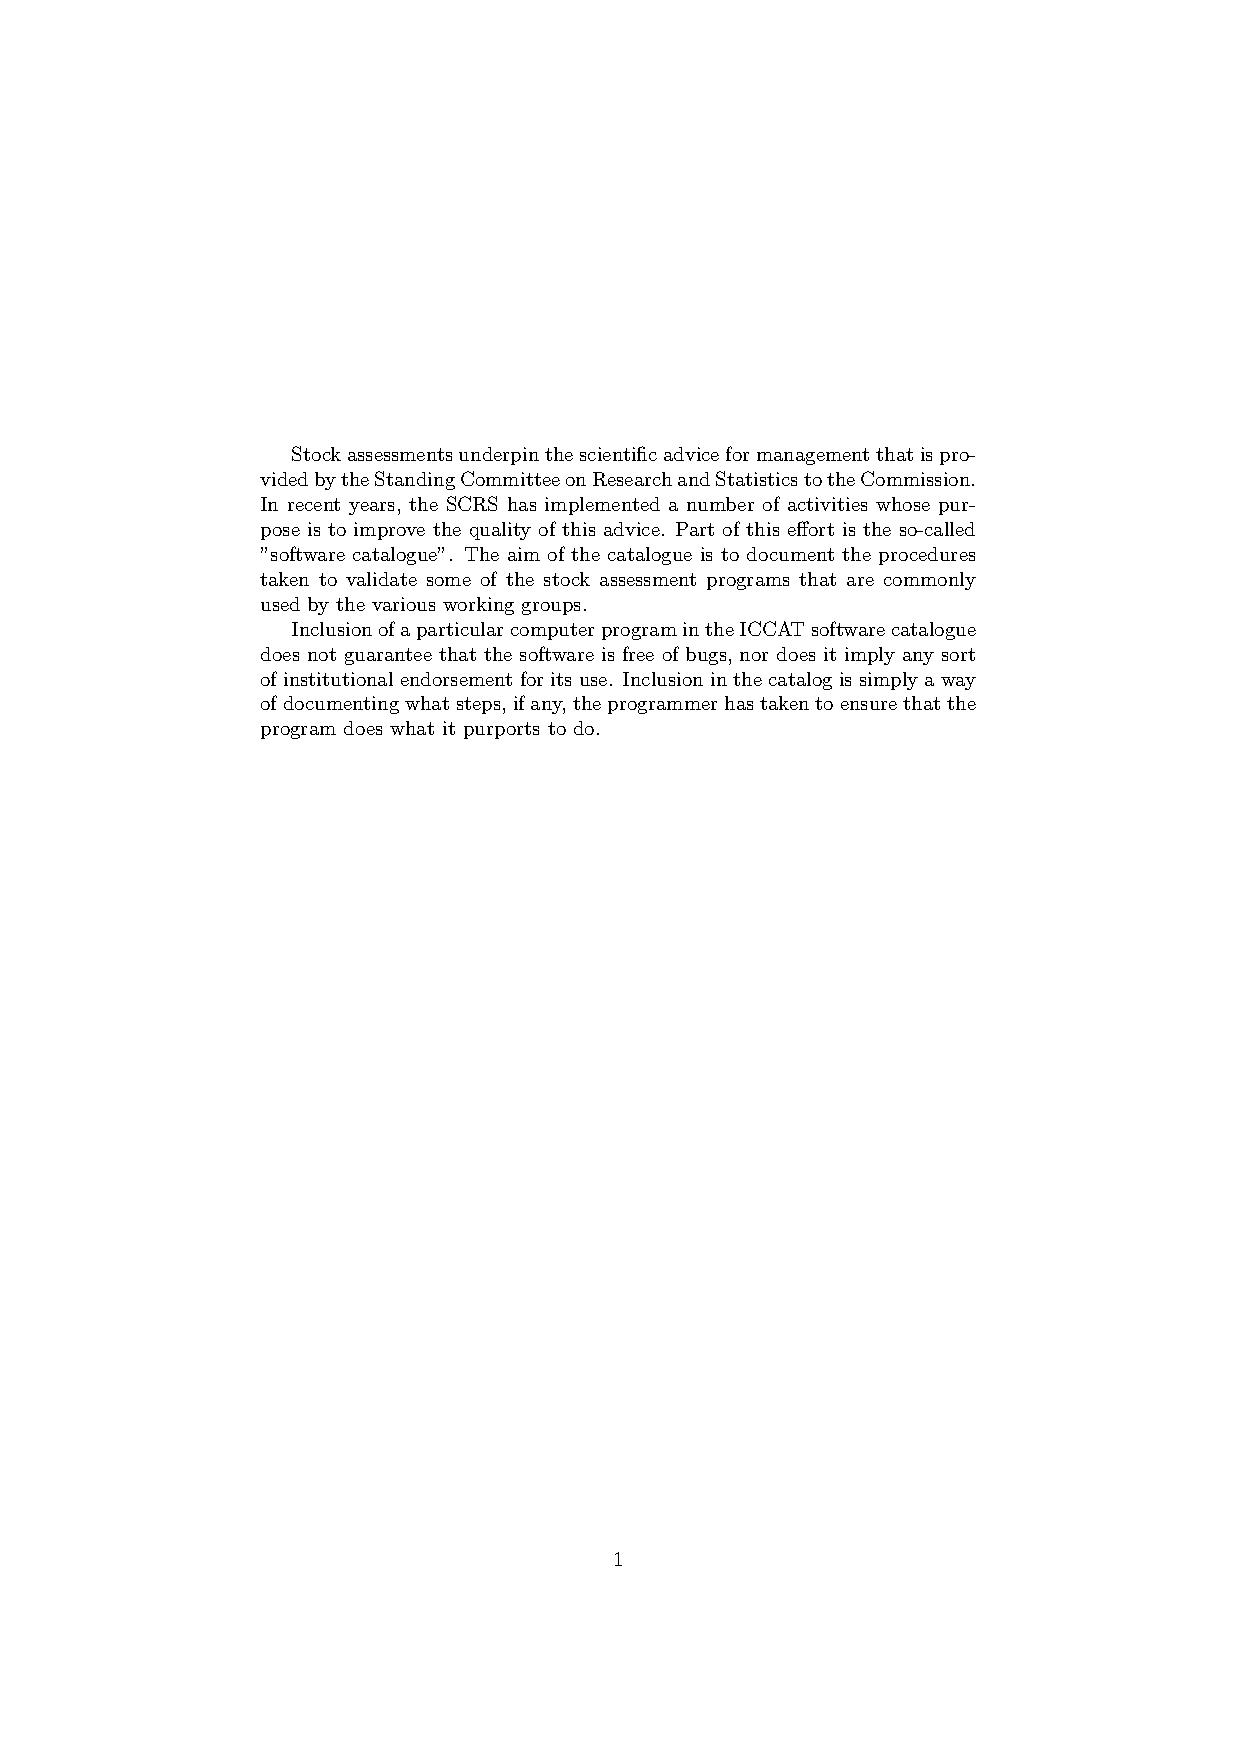
\includepdf[pages={1,2},lastpage=2]{application.pdf}

\subsection*{Related Issues}
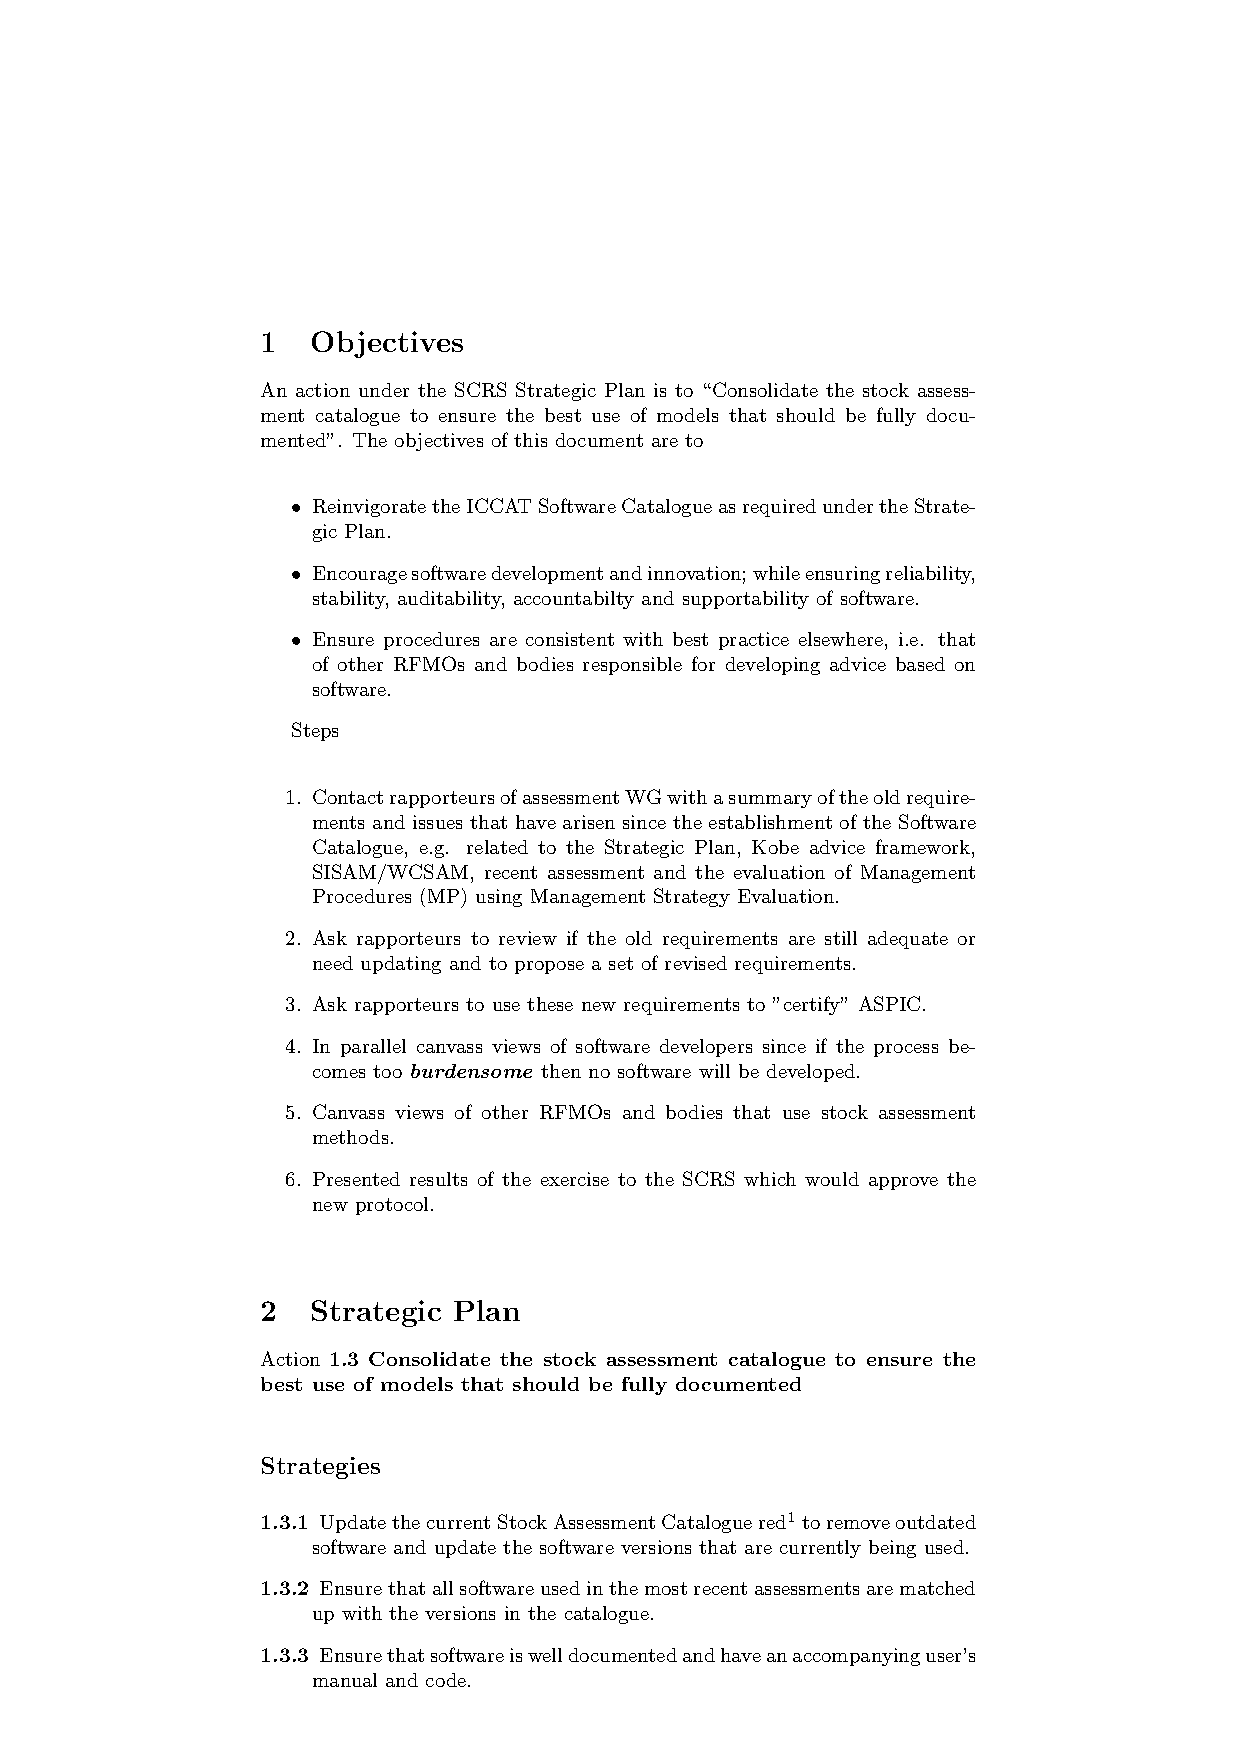
\includepdf[pages={1,2,3,4,5,6,7,8,9},lastpage=9]{softwareCatalogue.pdf}


\end{document}
